\subsection{Objektorientierte Programmierung}
In der Objektorientierten Programmierung mit Unity dreht sich alles um \textit{GameObjects}. Jedes Objekt in der Szene, egal ob sichtbar oder nicht, ist ein \textit{GameObject}. \textit{GameObjects} können verschiedene Komponenten haben, welche Eigenschaften definieren, also Daten speichern. Diese Komponenten sind jedoch nicht zu verwechseln mit den \textit{Components} aus dem datenorientierten Ansatz von Unity. Die Komponenten im objektorientierten Ansatz haben jeweils eine \texttt{Start} und eine \texttt{Update} Methode welche das Verhalten definieren. Die \texttt{Start} Methode wird einmalig vor dem ersten Aufruf der \texttt{Update} Methode ausgeführt. Die \texttt{Update} Methode läuft einmal pro ausgegebenem Bild. \hyperref[lstItemKomponente]{Listing \ref*{lstItemKomponente}} zeigt die Item Komponente des Item \textit{GameObjects}.
\begin{lstlisting}[style=code, caption={[Item Komponente im objektorientierten Ansatz]Item Komponente im objektorientierten Ansatz. Es speichert die Position und seine ID. In der \texttt{Update} Methode bewegt sich das Item linear zu der übergebenen Position.}, label=lstItemKomponente]
public class Item : MonoBehaviour {
    private int2 pos;
    //Serialisiertes Feld für den Unity Editor
    [SerializeField] private int itemID;

    void Update() {
    	//Gegenstand wird zu der übergebenen Position pos bewegt
        transform.position = Vector3.Lerp(transform.position,
            new Vector3(pos.x, pos.y, -0.5f), Time.deltaTime * 2f);
    }

    public void SetPosition(int2 pos) {
        this.pos = pos;
    }
}
\end{lstlisting}
Wie man sieht, beinhaltet das \texttt{MonoBehaviour} nicht nur die Daten, sondern auch die Logik. Für ein Item benötigen wir zum einen die Position, wohin sich das Item bewegen soll, zum anderen speichern wir auch eine ID über die wir das Item ganz einfach identifizieren können. Das Attribut \texttt{SerializeField} (Zeile 5) zwingt Unity dazu, ein editierbares Feld im Editor zu erstellen an dem man die \texttt{itemID} setzen kann. Dadurch lassen sich vorgefertigte Items erstellen, welche unterschiedlich aussehen und man zusätzlich die Item ID setzen kann. Beispielsweise ist ein Eisenbarren quadratisch, hat ein silbernes Material und bekommt die ID drei. Diese vorgefertigten Items kann man dann zur Laufzeit erstellen.
\begin{figure}[H]
\centering
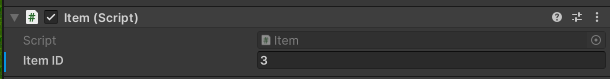
\includegraphics[scale=1]{Bilder/SerializeField.png}
\caption[\texttt{SerializeField}: Ein editierbares Feld in dem Unity Editor]{Ein editierbares Feld in dem Unity Editor. Das Feld wird durch ein \texttt{public} Attribut, oder dem \texttt{SerializeField} Flag erzeugt.}
\label{fig:SerializeField}
\end{figure}
Die \texttt{Start} Methode ist in diesem Fall nicht notwendig. Die \texttt{Update} Methode bewegt das Item langsam an die übergebene Position. \texttt{Time.deltaTime} (Zeile 11) gibt die Zeit in Sekunden von dem letzten Bild bis zu dem momentanen Bild an. Dadurch wird die Bewegung linear.\\
Ein weiterer Teil der Spielesimulation ist die Bewegung der Items über das Förderband. Das Förderband übergibt die Position an das Item und bestimmt daher, in welche Richtung sich das Item bewegen soll. \hyperref[lstConveyorKomponente]{Listing \ref*{lstConveyorKomponente}} beschreibt den Aufbau des Förderbandes.
\begin{lstlisting}[style=code, caption={[Förderband Komponente im objektorientierten Ansatz]Förderband Komponente im objektorientierten Ansatz. Es speichert die Ein- und Ausgabe des Förderbandes und alle Segmente die zu dem Förderband gehören. Das Förderband sorgt dafür, dass alle Items entlang des Förderbandes weiterbewegt werden.}, label=lstConveyorKomponente]
public class BeltPath : MonoBehaviour
{
    private List<ConveyorComponent> beltPath = new ();
    //Referenzen auf die Komponenten des GameObjects werden geholt
    private InputConveyorComponent input 
        = GetComponent<InputConveyorComponent>();
    private OutputConveyorComponent output 
        = GetComponent<OutputConveyorComponent>();
    private float timeToMove = 2f;

    public void Update()
    {
        timeToMove -= Time.deltaTime;
        //Bewegung der Items wird alle 2 Sekunden durchgeführt
        if(timeToMove > 0) return;
        var lastBelt = beltPath[^1];
        if (!ReferenceEquals(lastBelt.item, null)
            && ReferenceEquals(output.GetItem(), null)) {
            //Gegenstand von dem letzten Förderbandsegment
            //auf die Ausgabe legen
            var item = lastBelt.item;
            var itemComponent = item.GetComponent<Item>();
            itemComponent.SetPosition(output.GetPosition());
            output.SetItem(item);
            lastBelt.item = null;
        }
        //Gegenstände von hinten nach vorne um ein Segment verschieben
        for (int i = beltPath.Count-2; i >= 0; i--) {
            var thisConveyor = beltPath[i];
            var lastConveyor = beltPath[i + 1];
            if (!ReferenceEquals(thisConveyor.item, null)) {
                if (ReferenceEquals(lastConveyor.item, null)) {
                    //Item kann verschoben werden
                    var item = thisConveyor.item;
                    var itemComponent = item.GetComponent<Item>();
                    lastConveyor.item = item;
                    //Position des Items aktualisieren
                    itemComponent.SetPosition(lastConveyor.pos);
                    thisConveyor.item = null;
                }
            }
        }
        var firstConveyor = beltPath[0];
        input.SetOccupied(!ReferenceEquals(firstConveyor.item, null));
        if (!ReferenceEquals(input.GetItem(), null)
            && ReferenceEquals(firstConveyor.item, null)) {
            //Item wird von der Eingabe auf das erste Segment gelegt
            firstConveyor.item = input.GetItem();
            input.RemoveItem();
        }
        //Zeit wird wieder hochgestellt
        timeToMove += 2f;
    }
}
\end{lstlisting}
Für das Förderband wird eine Liste mit vorhandenen Segmenten, die Eingabe, die Ausgabe und eine Zeit gespeichert (Zeile 3 - 8). Die Zeit wird in der \texttt{Start} Methode initialisiert und die Ein- beziehungsweise Ausgabe wird über die Funktion \texttt{GetComponent} von dem \textit{GameObject} geholt. In der \texttt{Update} Funktion wird zunächst nur die \texttt{timeToMove} Variable herunter gezählt (Zeile 13). Sollte diese Variable unter Null fallen, werden alle Items von hinten nach vorne ein Segment weiter bewegt, sofern dies möglich ist. Ist die Ausgabe nicht belegt, wird ein vorhandenes Item in die Ausgabe gelegt (Zeile 17 - 26). In der Schleife werden die Items auf den einzelnen Segmenten weiterbewegt (Zeile 28 - 42) und wenn ein Item in der Eingabe liegt wird dieses auf das erste Segment weiterbewegt (Zeile 45 - 50). Immer wenn ein Item weitergegeben wird (egal ob an ein Segment, oder an die Ausgabe) wird auch die neue Position an das Item weitergegeben (Zeile 38). Durch das Bewegen der Items von hinten nach vorne verhindert man, dass sich Items nicht bewegen, obwohl sie es könnten.\\
Auf den Förderbändern sind Items sichtbare \textit{GameObjects}. In Gebäuden wird lediglich mit den ID's der Items gearbeitet, da man hier keine Objekte braucht. Items werden in der Ausgabe eines Gebäudes erstellt und von dort an das Förderband übergeben.  Die \texttt{Update} Methdode dafür zeigt \hyperref[lstCreateItemOOP]{Listing \ref*{lstCreateItemOOP}}.
\begin{lstlisting}[style=code, caption={[Erstellung eines Items im objektorientierten Ansatz]Erstellung eines Items im objektorientierten Ansatz. Wenn ein Förderband verbunden ist und ein Item erstellt werden soll, wird das passende \textit{GameObject} instanziert. Dieses wird dann an das Förderband übergeben.}, label=lstCreateItemOOP]
void Update()
{
    //Wenn die Ausgabe leer ist gibt es nichts zu tun
    if(itemID == -1) return;
    outputGameObject ??= BuildingDictionary.Instance
        .GetGameObjectAtPosition(pos);
    if (ReferenceEquals(outputGameObject, null) ||
        !outputGameObject.TryGetComponent(out InputConveyorComponent input))
        return;
    //Wenn die Eingabe des Förderbandes belegt ist wird auch keine
    //Änderung vorgenommen
    if(input.IsOccupied() || !ReferenceEquals(input.GetItem(), null))
        return;
    var itemGameObject = Items.INSTANCE.GetItem(itemID);
    //Item wird erstellt
    var item = Instantiate(itemGameObject, new Vector3(pos.x, pos.y, -0.5f), Quaternion.identity);
    item.transform.localScale = new Vector3(0.5f, 0.5f, 0.5f);
    var itemComponent = item.GetComponent<Item>();
    itemComponent.SetPosition(pos);
    var inputConveyorComponent = outputGameObject
        .GetComponent<InputConveyorComponent>();
    //Der Eingabe wird das Item zugewiesen
    inputConveyorComponent.SetItem(item);
    //Item wird aus der Ausgabe entfernt
    itemID = -1;
    itemCreated = true;
}
\end{lstlisting}
Da man sich im objektorientierten Ansatz, ohne weitere Vorkehrungen, immer auf dem \textit{Main Thread} befindet, lassen sich die Items direkt erstellen und der Eingabe übergeben. Das Zerstören von Items, also der Fall wenn Items von einem Förderband in ein Gebäude übergeben werden, funktioniert sehr ähnlich zu dem Erstellen von Items.